\section{Head-Mounted Display Evaluation}
\label{result:hardware}
In order to get insights into possibilties and limitations of VR hardware today, two different HMDs were evaluated. The selection were based on avaliability of the HMDs and previous experience by the author. The focus of the evaluation lies in portability, DOF, possible interactions and support by Unity VR Editor. The selected devices are:
\begin{itemize}
  \item HTC Vive
  \item Google Daydream
\end{itemize}
\subsection{Hardware specification}
Table \ref{table:result:hardware:spec} consist of the hardware specification from the selected devices.
\begin{table}[]
\centering
\caption{Hardware specification of HTC Vive and Google Daydream}
\label{table:result:hardware:spec}
\begin{tabular}{|l|l|l|}
  \hline
                       & \textbf{HTC Vive}\footnote{https://www.vive.com/eu/product/}  & \textbf{Google Daydream}\footnote{https://vr.google.com/daydream/headset/}          \\\hline
Resolution             & 1200 x 2160 pixels & (Google Pixel) 1080 x 1920 pixels \\\hline
Nr of Controllers      & 2                  & 1                                 \\\hline
Controller DOF         & 6                  & 6                                 \\\hline
Room tracking          & Yes                & No                                \\\hline
Wireless               & No                 & Yes                               \\\hline
Phonebased             & No                 & Yes                               \\\hline
Unity EditorVR Support & Yes                & No                                \\\hline
\end{tabular}
\end{table}
\subsection{Test Analysis}
Initial tests of the different HMDs were performed by the author to gain insights of what each setup had to offer. This section contains insights and experiences from the author based on usage of the HMDs.
\subsubsection{HTC Vive}
\label{result:hardware:vive}

\begin{figure}
  \centering
  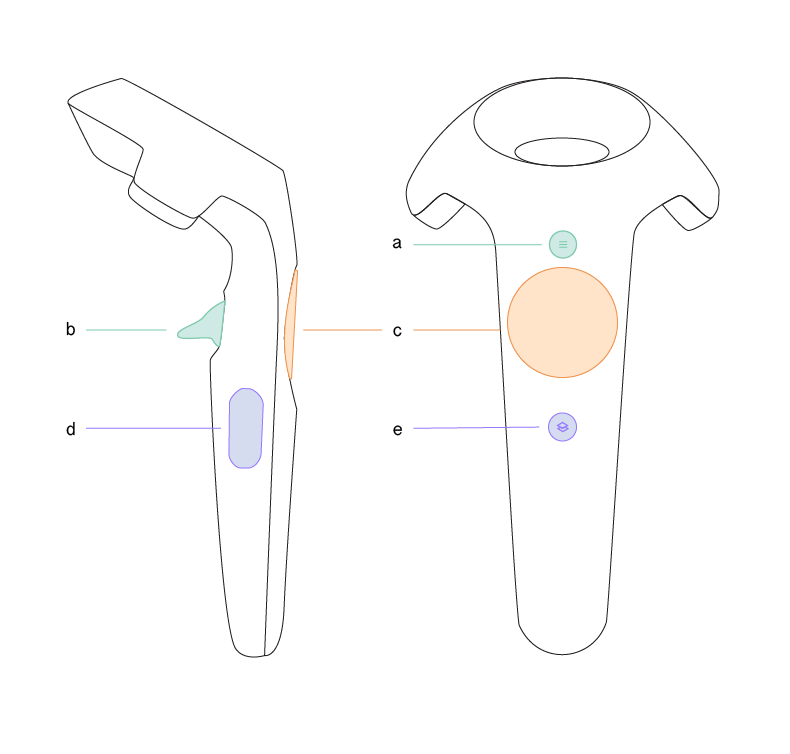
\includegraphics[width=.8\linewidth]{vive_controller.png}
\caption{Outline of buttons from HTC Vive controller.}
\label{fig:result:hardware:vive:controller}
\end{figure}

The HTC Vive is the most powerful and has the best resolution of the selected devices, which allows for more complex environments and experiences. It has two wireless 6-DOF controllers that consists of an application button (Label \ref{fig:result:hardware:vive:controller}.a), a trigger (Label \ref{fig:result:hardware:vive:controller}.b), a thumb touchpad (Label \ref{fig:result:hardware:vive:controller}.c), two squeeze buttons (Label \ref{fig:result:hardware:vive:controller}.d),  and a menu button (Label \ref{fig:result:hardware:vive:controller}.e). Its biggest asset however is the room-tracking of both the HMD and the controllers with which the user can perform complex interactions with high precision. With support for Unity EditorVR and its API the Vive can be used to alter existing Unity projects.
These features does however come with a cost, both in terms of portability and financially. The system relies on a standalone state of the art computer to run applications and experiences, which is connected with wires to the HMD. In order to track the users controllers and HMD, two sensors have to be placed in the room which creates a bounding box of the tracked area. These sensors have to be mounted on a wall or onto a stand and then callibrated, which in itself is a five-minute process. Its high pricetag combined with the space required limits the number of devices that will be present in a studio or office.
This device is suited for high-precision interactions in complex scenes and environments, it also works as a great test suite for iterations of an experience as it could allow changes to the experience that is being tested.


\subsection{Google Daydream}

\begin{figure}
  \centering
  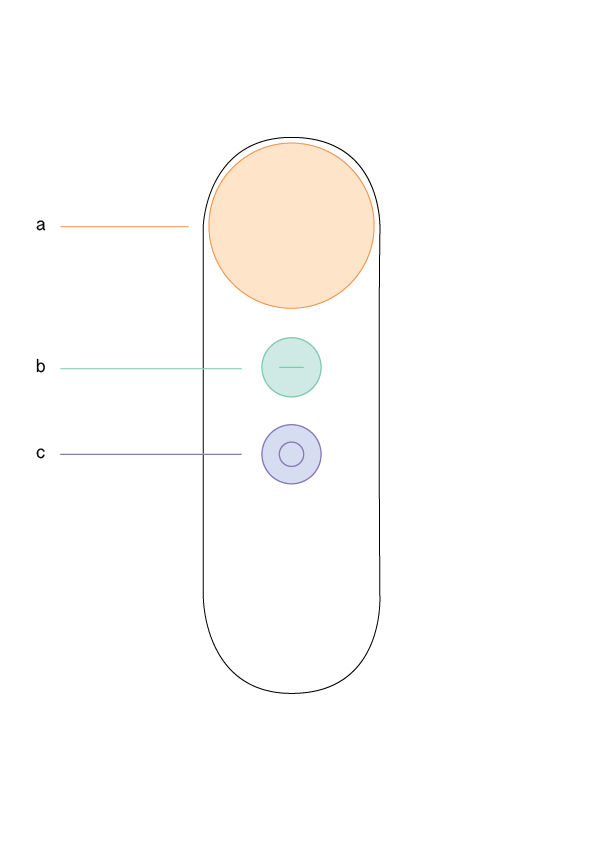
\includegraphics[width=.5\linewidth]{daydream_controller.png}
\caption{Outline of buttons from Google Daydream controller.}
\label{fig:result:hardware:daydream:controller}
\end{figure}

\label{result:hardware:daydream}
Daydream is created by Google as a phone-based VR device that works without external support. Only a selected number of mobile devices are currently officially supported as "Daydream-ready", and the performance of the setup relies on the specification of the mobile device. The device consist of a HMD that is tracked with internal sensors and one wireless 3-DOF controller. The controller offers a clickable thumb touchpad (Label \ref{fig:result:hardware:daydream:controller}.a), a application button (Label \ref{fig:result:hardware:daydream:controller}.b) and a syste menu button (Label \ref{fig:result:hardware:daydream:controller}.c). The biggest advantage with this device out of the list of selections is the portability and space required to operate. This device can be used while at a regular desk at an office, at a pricepoint that makes it individually avaliable. This setup suffers from some shortcommings as well. It struggles when it comes to complex environments because of limited processingpower in the mobile device. It also has a limited set of interaction capabilities due to the fact that the internal sensors in the HMD and the controllers cannot track relative motions in space, only changes in movement. It is not supported by Unity EditorVR which limits the functionality in practice to something like a sandbox, where the created environments stays within the enclosed system of the device or application.
This setup works best for rough tests and basic interaction pattern, for simple prototyping and tests of elements and its basic properties. With this approach the portable and simple setup can be utilized by professionals at their current workstation.

\subsection{Unity VR Editor}
The approach of using a HMD setup to alter a VR project is designed from an API that was released for the 3D game engine Unity in late december of 2016\footnote{https://blogs.unity3d.com/2016/12/15/editorvr-experimental-build-available-today/}. The tool is called Untiy EditorVR and allows altering of an open Unity project from a HTC Vive or Oculus Rift.
